\chapter{Egy frekvenciaváltó tervezése}

\paragraph{}
Tesla 1888-ban bemutatott három fázisú indukciós motorjával, nyilvánvalóvá vált, hogy az ilyen típusú gépek megbízhatóbbak és gazdaságosabbak tudnak lenni, mint az egyenáramú társaik. Jelentős hátrányuk azonban, hogy a vezérlésükhöz három fázisú feszültséget kell előállítani, mely akkoriban csak egy szintén három fázisú generátor segítségével volt megoldható. Manapság a három fázisú teljesítmény a villamos hálózatnak köszönhetően rendelkezésre áll, azonban még így is vet fel problémákat ezen motorok üzemeltetése.

\paragraph{}
A frekvenciaváltó egy olyan eszköz mely váltakozó áramú bemenetből váltakozó áramú kimenetet állít elő, mint ahogy a neve is mutatja, más frekvenciával vagy akár feszültséggel, mint a bemenet. Erre azért van szükség, mert a meghajtani kívánt folyamatnak nagyon valószínű, hogy más igényei vannak, mint amit a hálózat önmagában képes biztosítani. Értem ez alatt azt, hogy közvetlen összeköttetés esetén a motorunk $50\ Hz-el$, vagy ennek egész számú hányadosával tudna forogni, illetve ennek a paraméter a befolyásolása csak a motor fizikai módosításával lehetséges, azaz más pólus pár számú motort kell beépíteni. Természetesen mint az ipar és az élet minden szegmensében itt is célunk a feladat minél hatékonyabb végrehajtása. A világon a teljes villamosenergia felhasználás mint egy $25\ \%-$-át adják a villamos hajtások és ez a szám folyamatosan nő (például az elektromos közlekedés tér nyerésével). Az igény tehát nyilvánvaló ezen eszközöknek folyamatos fejlesztésére.

\begin{figure}[!h]
	\centering
	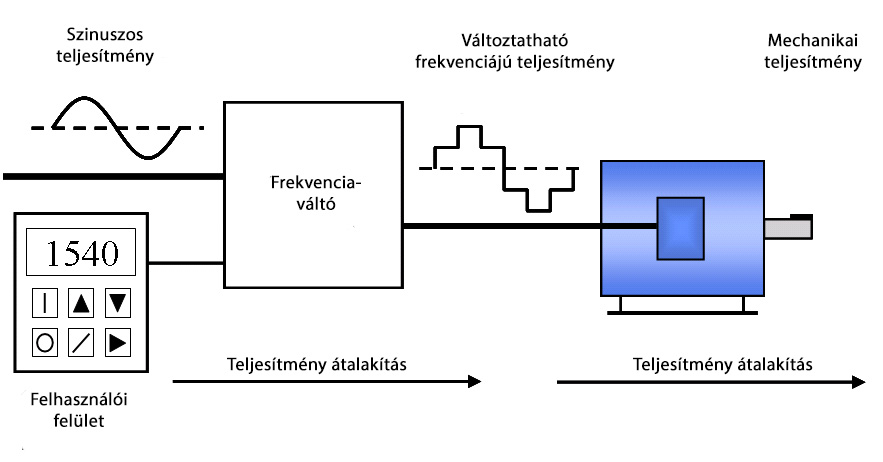
\includegraphics[width = 0.8\textwidth]{figures/VFD_System.jpg}
	\caption{A frekvenciaváltó szerepe} 
	\label{fig:vfd_system}
\end{figure}

\paragraph{}
Az eszköz feladatát jól összefoglalja \aref{fig:vfd_system} ábra. A hálózatból érkező teljesítményt, a felhasználó által megadott paraméterekkel átalakítjuk, majd a terhelő gépet meghajtjuk vele. A modern hajtások azért ennél már jóval szofisztikáltabb működésre is képesek, gondoljunk itt akár táv felügyeletre, identifikációra, vagy esetleg akár vezeték nélküli hozzáférésre. Szükség lehet konstans fordulatszám, vagy konstans nyomaték tartásra, esetleg pontos pozíció szabályozásra. Más igények mutatkoznak egy szállító szalag, egy víz pumpa, vagy egy szellőztető ventilátor esetén.

\paragraph{}
A korábban az ilyen teljesítmény átalakítási feladatokat elektromechanikus berendezésekkel oldották meg, nevezetesen egy motor és generátor párral, ahol is a megfelelő pólus pár arány kiválasztásával a frekvenciát módosítani lehetett. Amennyiben szükséges volt feszültség módosítás is, megfelelő áttételű transzformátor segítségével valósították meg. Ennek a megoldásnak hátránya a nagy teljesítmény esetén nagy méretű villamos gép, ennek megfelelően a kicsi teljesítmény-sűrűség. A megbízhatóságot csökkenti a mozgó alkatrészek jelenléte és folyamatos igénybevétele, illetve a nagy forgó tömeg is hordoz magában veszélyeket. Ezt követően megjelentek a vákumcsöves eszközök, azonban az igazi áttörést a teljesítmény-elektronikai félvezető elemek megjelenése okozta.

\paragraph{}
Ezek a modern eszközök már nem tartalmaznak mozgó alkatrészt (feltéve persze, hogy a reléket és kontaktorokat nem számítjuk mozgó alkatrésznek). A félvezető technológia fejlődésével egyre nagyobb és nagyobb teljesítmény-sűrűségeket tudunk elérni. A jövőben nagy lehetőség rejlik a $SiC$ - szilícium-karbid alapú félvezető eszközök használatában. Ezen típusú eszközök a napjainkban szokásosnál sokkal nagyobb kapcsolási frekvenciát is megengednek, így jelentősen csökkentető a beépített mágneses anyag tömege, ezáltal az eszköz mérete is. A FET-eken a maradék feszültség értéke is sokkal kisebb, mint az IGBT-ken, így a kapcsolási veszteség is kisebb lehet a nagyobb kapcsolási frekvencia ellenére. A $SiC$ alapú felvezetők sokkal magasabb hőmérsékleten is üzem képesek tudnak maradni, akár $200 °C$ körüli üzemi hőmérséklet is elérhető, aminek köszönhetően a hűtés hatékonyabbá válik, mivel a hűtő közeg és az eszköz között nagyobb lesz a $\Delata{}T$ hőmérséklet különbség. A mi frekvanciaváltóinkban még IGBT-k találhatóak, de a technológia fejlődésével a jövőben előfordulhat $SiC$ alapú frekvenciaváltó készítése is.

\begin{figure}[!h]
	\centering
	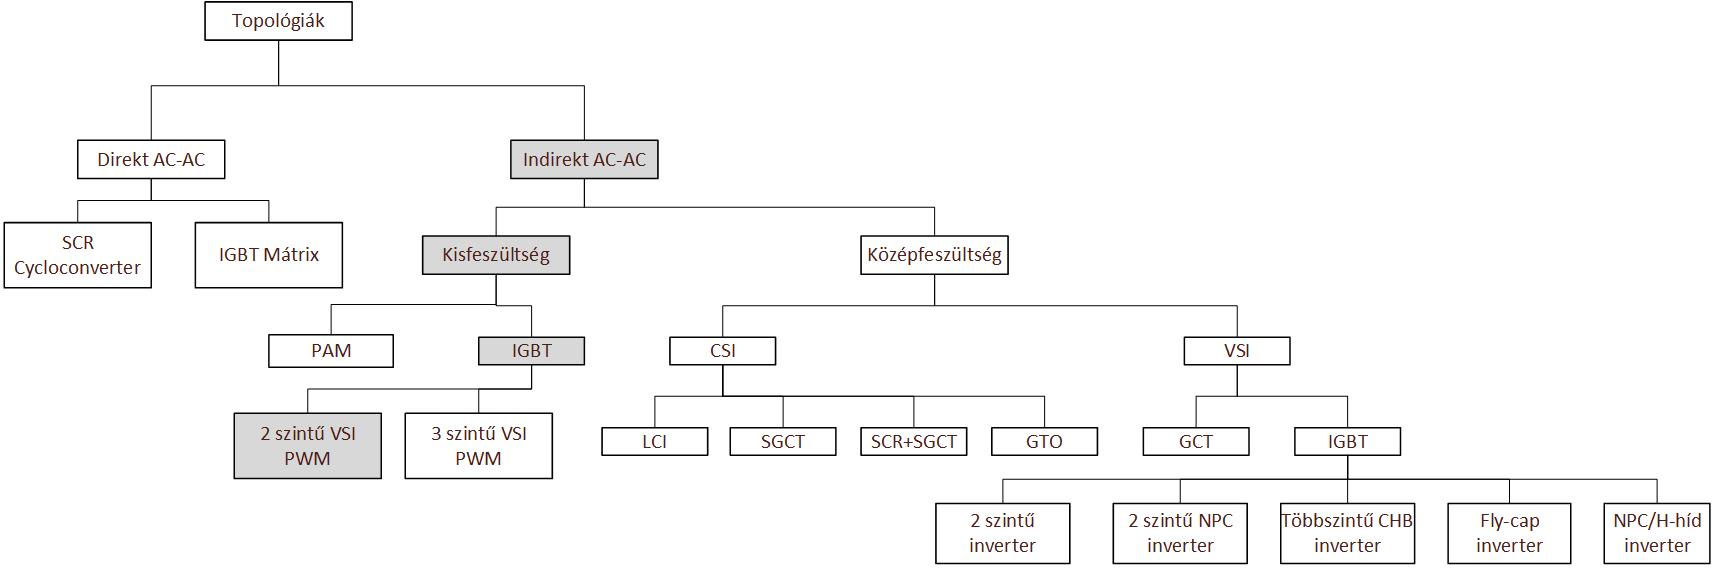
\includegraphics[width = \textwidth]{figures/topologies.jpg}
	\caption{A frekvenciaváltó típusok} 
	\label{fig:topologies}
\end{figure}

\Aref{fig:topologies} ábrán láthatjuk a napjainkban elterjedt inverter típusokat. Az ábrában szürkével kiemeltem a Hyundai által fejlesztett típust.

\section{Termék specifikáció}

A Hyundai által jelenleg fejlesztett frekvenciaváltó család kis feszültségű, általános célú PWM vezérlet IGBT kapcsoló elemű 2 szintű inverteres frekvenciaváltó, passzív front-end-el, azaz a hálózatra nem tud visszatáplálni. \Aref{fig:family} táblázatban látható a jelenleg fejlesztett termék család. \todo{wikipédia hivatkozás}

\begin{table}[]
\centering
\begin{tabular}{|c|c|c|c|l}
\cline{1-4}
\textbf{Név} & \textbf{Teljesítmény (kW)} & \textbf{Áram (A)} & \textbf{Tömeg (kg)} &  \\ \cline{1-4}
\multirow{4}{*}{\textbf{FR1}} & 0,55 & 3,7 & \multirow{4}{*}{6} &  \\ \cline{2-3}
 & 0,75 & 4,8 &  &  \\ \cline{2-3}
 & 1,1 & 6,6 &  &  \\ \cline{2-3}
 & 1,5 & 8 &  &  \\ \cline{1-4}
\multirow{3}{*}{\textbf{FR2}} & 2,2 & 11 & \multirow{3}{*}{10} &  \\ \cline{2-3}
 & 3,7 & 18 &  &  \\ \cline{2-3}
 & 5,5 & 25 &  &  \\ \cline{1-4}
\multirow{2}{*}{\textbf{FR3}} & 7,5 & 31 & \multirow{2}{*}{20} &  \\ \cline{2-3}
 & 11 & 48 &  &  \\ \cline{1-4}
\multirow{3}{*}{\textbf{FR4}} & 15 & 62 & \multirow{3}{*}{37,5} &  \\ \cline{2-3}
 & 18,5 & 75 &  &  \\ \cline{2-3}
 & 22 & 88 &  &  \\ \cline{1-4}
\multirow{3}{*}{\textbf{FR5}} & 30 & 114 & \multirow{3}{*}{66} &  \\ \cline{2-3}
 & 37 & 140 &  &  \\ \cline{2-3}
 & 45 & 170 &  &  \\ \cline{1-4}
\multirow{2}{*}{\textbf{FR6}} & 55 & 211 & \multirow{2}{*}{108} &  \\ \cline{2-3}
 & 75 & 261 &  &  \\ \cline{1-4}
\end{tabular}
\caption{A fejlesztés alatt álló termékpaletta}
\label{fig:family}
\end{table}

\paragraph{}
Azt, hogy a termék milyen széles területét lefedi az iparnak, jól jellemzi, hogy az ezt leíró dokumentum 52 különböző tételt különböztet meg. A teljesség igénye nélkül a felvevő piac néhány szelete:

\begin{itemize}
	\item{Nagyfeszültségű légkondícionálók}
	\item{Élelmiszeripar}
	\item{Textilipar}
	\item{Szállító szalagok}
	\item{Csomagolás és cimkézés}
	\item{Nyomtatás}
	\item{Gépi megmunkálás}
	\item{Autóipar}
\end{itemize}

\paragraph{}
A hardveres funkcionalitás nagyjából megegyezik minden esetben, az igazán nagy különbség az egyes területek között a szoftver funkcionalitásában van. Egy szállítószalag esetében fontos a pontos fordulatszám tartása, vagy a pontos pozíció beállítása, míg más felhasználás esetében a pontos nyomaték szabályozás lehet fontos, ilyen lehet például a villamos vontatás.

\paragraph{}
Amennyiben külön nincsen jelölve, a dolgozat a továbbiakban az FR1 (Frame 1) kódjelű, legkisebb frekvenciaváltóra hivatkozik a példák esetében.

\section{Az eszköz felépítése}

\paragraph{}
A frekvenciaváltó egyenirányítja a bejövő hálózati feszültséget, egy köztes energia tárolóban, az ún. \emph{DC-link} kondenzátorban tárol némi energiát, hogy a feszültség lengését alacsonyan tartsa, majd egy kimeneti inverterrel előállítja a szükséges jel alakot. Ezt a vázlatot láthatjuk \aref{fig:vfd_schema} ábrán, kiemelve a hálózatot modellező ellenállást és induktivitást.

\begin{figure}[h]
	\centering
	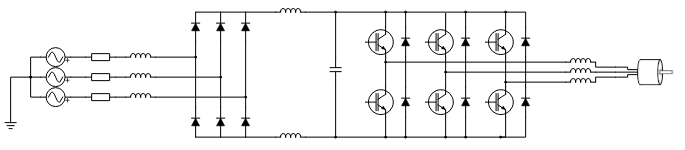
\includegraphics[width = \textwidth]{figures/VFDschematic_choke.png}
	\caption{A frekvenciaváltó egyszerű felépítése} 
	\label{fig:vfd_schema}
\end{figure}

\paragraph{}
Itt természetesen csak egy vázlatos ábrázolás látató, ezen nem szerepelnek a meghajató elektronikák, a vezérlés, a mérések, és még sok más. Jól látható azonban, hogy a folyamatra egyedül a félhidak vezérlésével tudunk hatni. A Frame 1-ben a kimeneti IGBT-k és diódák egy tokban vannak, egy Semikron SKiiP 24NAB12T4V1 modulban. \cite{sutozoli}

\section{A szükséges kompetenciák}

A felépítés alapján elmondható, hogy egy ilyen termék összeállítása nagyon bonyolult feladat, sok területet lefed, sok féle kompetenciára van szükség. A teljesítmény elektronikai elemek és kapcsolálsok megtervezése gyakorlatilag csak az első gondolat. Ezen túl szükséges még a termikus méretezés, a vezérlő elektronikák tervezése, a különböző mérések megvalósítása. Amikor már ezzel is készen vagyunk, akkor a frekvenciaváltó tervezése elektronikai szempontból késznek mondható. Nem szabad megfeledkezni azonban arról, hogy ez egy készülék, melynek a mechanikus felépítéséről is gondoskodni kell. Itt kerülnek képbe a konstrukcióval foglalkozó gépész kollégák.

\begin{figure}[h]
	\centering
	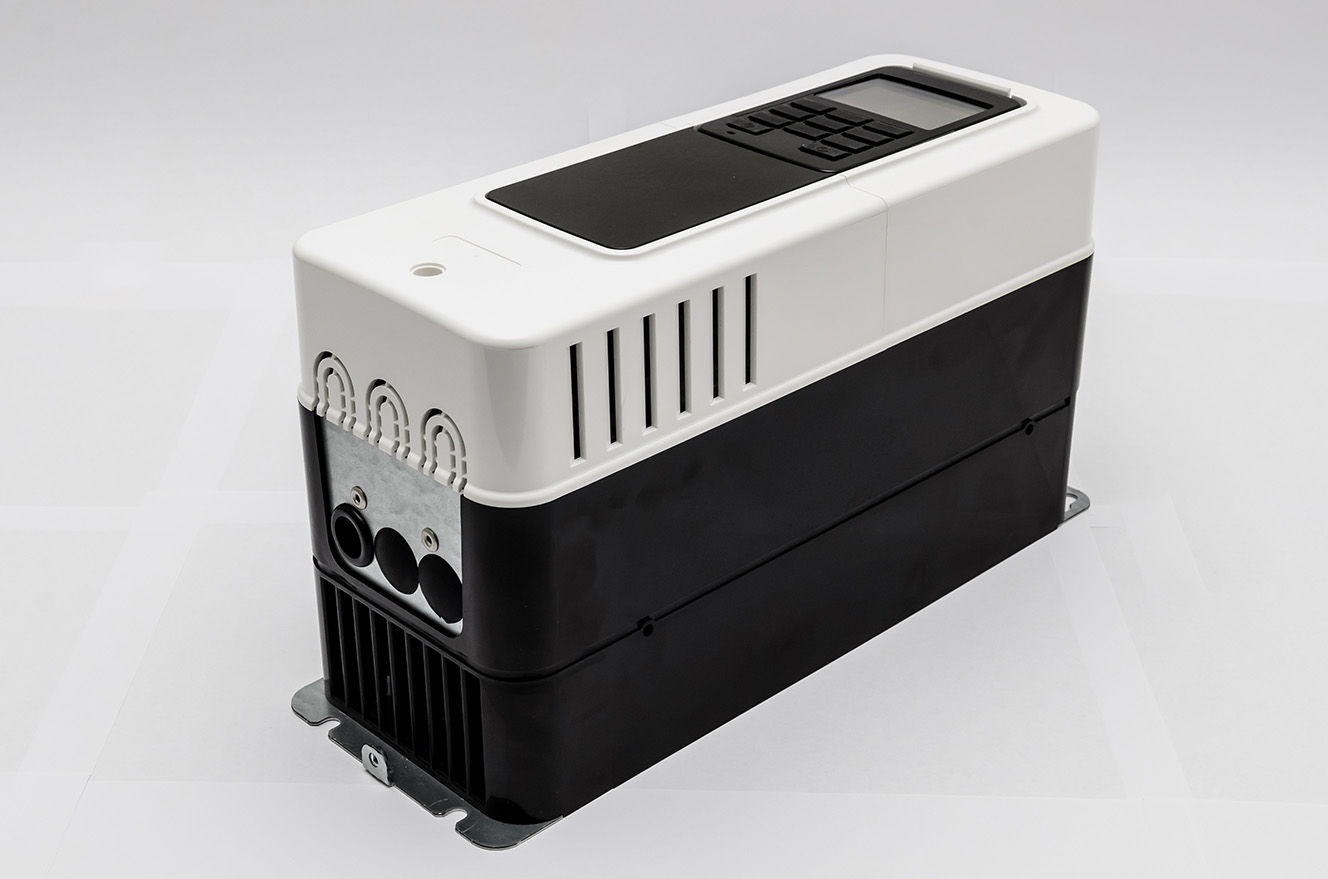
\includegraphics[width = 0.8\textwidth]{figures/n700_proto.jpg}
	\caption{Az elkészült Frame 1 prototípus} 
	\label{fig:n700_proto}
\end{figure}

\paragraph{}
A feladat már eddig is kellőképpen összetett volt, de a termékünk még mindig nem működő képes. Hiányzik belőle a szoftver, mely önmagában nagyon szerteágazó munka. Először is elő kell állítani a megfelelő szabályzókat, melyek segítségével elő tudunk állítani szinuszos kimenetet, gondoskodni kell a kapcsoló elemek vezérlő jelének megfelelő modulációjáról. Foglalkozni kell a magasabb szintű funkcionalitás megvalósításával, a különböző kommunikációs vonalak kezelésével, magának a rendszernek a menedzselésével. A HMI\footnote{Human-Machine Interface}-n is meg kell jelenteni információt, biztosítani kell lehetőséget a beavatkozásra. Amennyiben úgy gondolná az olvasó, hogy ez még nem annyira bonyolult, akkor figyelmébe ajánlom a PC-s szoftvert, melyet szintén különös gonddal el kell készíteni, ha egy jól használható terméket kívánunk előállatni, hiszen a felhasználó ezen keresztül fogja a legkönnyebben felkonfigurálni igényei szerint az eszközt.

\todo[inline]{Félbehagyott gondolat}

\begin{figure}[h]
	\centering
	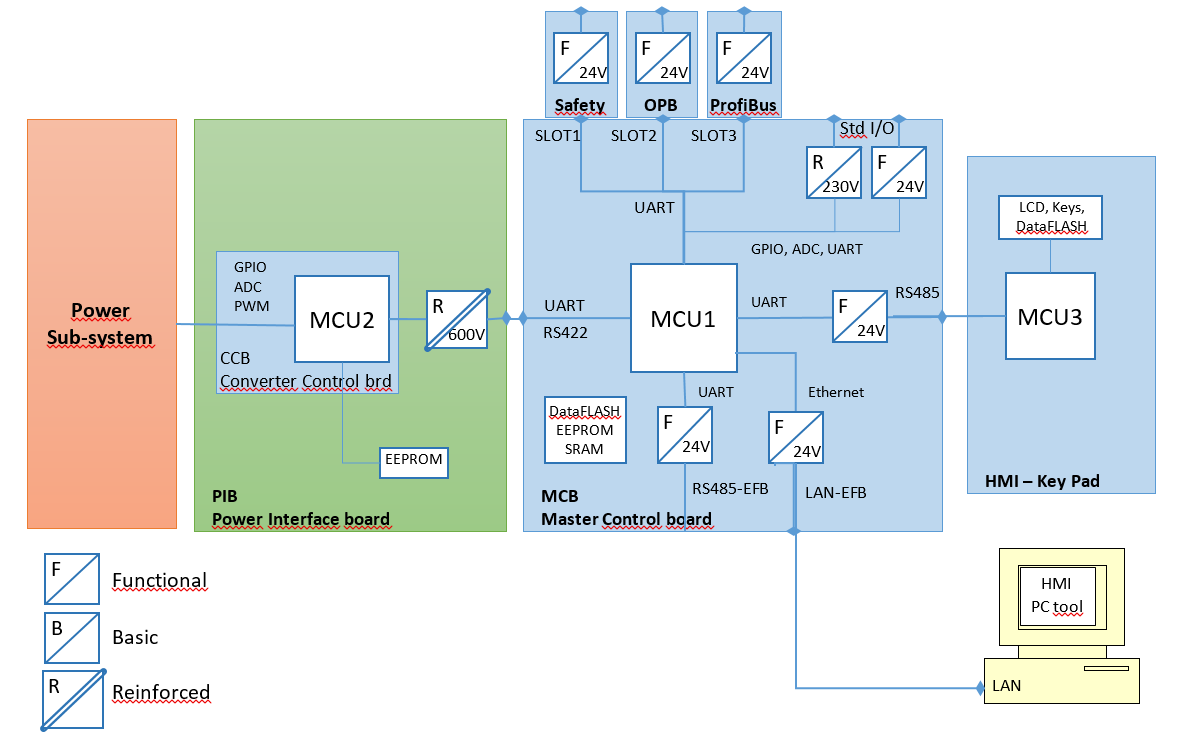
\includegraphics[width = \textwidth]{figures/architect.png}
	\caption{A vezérlő elektronika blokkvázlata} 
	\label{fig:hw_architect}
\end{figure}

\paragraph{}
\Afigref{hw_architect} ábrán látható a különböző elemek kapcsolata, illetve a kommunikáció közöttük. A CCB feladata a teljesítmény átalakítás közvetlen irányítása. Ez a kártya végzi az analóg méréseket, és ezen mérések, illetve a beérkező alapjel figyelembe vételével előállítja az IGBT-ket vezérlő PWM jeleket. A szoftveres védelmekről is ez a szint gondoskodik. A következő az MCB, mely az egyel magasabb szintű vezérlésért felel. Ez jelenti a kommunikációt más eszközökkel, a különböző terepi buszukon, etherneten, vagy RS-485-ön. Rendelkezik továbbá általános célú digitális és analóg be és kimenetekkel, melyek működése felhasználói igények szerint testre szabható. Ez az eszköz felelős a számítógépes konfiguráló szoftverrel való kommunikációért, valamint a HMI vezérléséért is. A fejlesztett HIL szimulátor szempontjából ez a három elektronika bír szereppel, ezek közül a HMI csak közvetetten, mivel az MCB-n keresztül kapcsolódik a rendszerhez.

\chapter{A fejlesztés folyamata}

A teljesítmény elektronikai eszközök fejlesztésének a nehézsége abban rejlik, hogy a kisebb teljesítményű modell nem feltétlenül viselkedik úgy, mint nagy áramú társa. A fenti leíráson az is jól látszik, hogy bizonyos folyamatok párhuzamosíthatóak. A szoftver fejlesztés elkezdődhet a nagy áramú elektronika tervezésével együtt, illetve a vezérlő elektronikák is tervezhetőek a kezdeti specifikációk, illetve a a kapcsolódási pontok definiálása után. A fejlődő szoftver teszteléséhez azonban elengedhetetlen, hogy a beágyazott eszköz megkapja a szükséges gerjesztéseket a külvilágtól. Amíg nem áll rendelkezésre a valós eszköz, addig ezt egy szimulátorral vagyunk kénytelenek megvalósítani. Ez lehet akár egy Hardware-in-the-Loop szimulátor. Egy ilyen eszköz jól jön azonban amikor már a valós frekvenciaváltó is rendelkezésre áll. Az egyes szoftver módosításokat célszerű kipróbálni ezen az eszközön először, mert egy hiba könnyedén végzetes következményekkel járhat a valós inverteren.

\section{Különböző szimulációs eljárások összehasonlítása}

\todo[inline]{Logikai bukfentc, korábban már van HIL, de csak most kezdem kibontani ,hogy mi is az.}

\paragraph{}
Jól látható tehát, hogy egyértelmű igény mutatkozik valamilyen szimulációs eljárás használatára a fejlesztés minden szakaszában. Természetesen mint minden problémánál, itt is több megközelítés közül választhatunk. Ami mindenképp közös az eljárásokban, hogy a kiváltott hardver-elemek matematikai modelljeit fel kell állítani, azok helyességéről meg kell győződni. A modellezés pontossága és az erőforrás igény között azonban meg kell találni az adott alkalmazásnak és annak szükségleteinek megfelelő kompromisszumot. Elengedhetetlen követelmény azonban, hogy az irányító elektronika szempontjából a modell teljesen transzparens legyen, egyébként nem tudunk reprezentatív következtetést levonni a működés helyességével kapcsolatban. Ez azt jelenti, hogy ugyan azokon az interfészeken keresztül tudjunk a szimulátorral interakcióba lépni, ugyan azokat a válaszokat kapja a szakasztól, mint amit a valóságban is fog kapni, valamint az időzítések is egyezzenek meg az igazi eszközön tapasztaltakkal.

\paragraph{}
Joggal merül fel a gondolat, hogy asztali számítógépen futtassuk a kifejlesztett modellt, hiszen szokványosan használjuk PC-nket különböző számítások elvégzésére. Ezzel módszerrel azonban nagyon hamar problémákba ütközünk. Az első követelmény, hogy rendelkezzen a számítógépünk adat gyűjtő modullal (DAQ - Data Aqusition Module), mely segítségével tudunk mérni és előállítani analóg és digitális jeleket. Ilyen eszközöket lehet kereskedelmi forgalomban kapni, kérdéses azonban a biztosított sávszélesség, a számítógéppel való kommunikáció sebessége, illetve a költsége a vásárolt hardvernek. Ezen felül korlát még az időzítések betartása. Nem is biztos, hogy a számítógépünk valós időben el tudja végezni a szimulációhoz szükséges matematikai műveleteket, de ha feltételezzük, hogy igen, az egzakt és konzisztens lépésköz egy általános célú asztali számítógépen nem garantálható az operációs rendszer sajátságaiból adódóan. Ennek megoldására állnak rendelkezésre valós idejű megoldások, például valós idejű futást támogató Linux kernel, melyet hasonló célra fejlesztettek ki. A számítógép hardveres konfigurációja is korlátot jelent, mert hiába növeljük a processzor teljesítményt, egy ponton túl ($1 - 10 \mu{}s$) a memória hozzáférések késleltetése miatt nem tudunk kisebb szimulációs lépésközt biztosítani.

\paragraph{}
A következő lehetőség saját beágyazott hardver fejlesztése, mely emulálja a valós teljesítmény elektronikát. Ebben az esetben teljesen testre tudjuk szabni a kapcsolódási pontokat, elő tudjuk állítani azokat a jeleket, melyeket vár a vezérlő elektronika, pontosan úgy ahogy szeretnénk. Előnye a beágyazott processzornak, hogy architektúrájából adódóan garantált futásidőt lehet elérni. A teljesítménye azonban korlátozott az asztali számítógéphez képest, bár, mivel csak egy specifikus feladatot kell végrehajtani, akár még versenyezhet is futásidőben az asztali számítógéppel. Fentiek miatt ez a megoldás leginkább funkcionális tesztek végrehajtására alkalmas, precíz, kvantitatív tesztek végzésére korlátozottan.

\paragraph{}
A harmadik út - amit részletesebben megvizsgálok dolgozatomban - az FPGA alapú hardware-in-the-loop szimulátor tervezése. Bár a fejlesztési idő és a hardver költsége szintén magas lehet, az FPGA architektúrájából adódóan, nevezetesen, hogy létre tudjuk benne hozni az éppen szükséges számításokat elvégző hardvert, rendkívül gyors futásidő érhető el. Ráadásul a PC-vel ellentétben itt az FPGA teljesítményének és órajelének növelésével egyre nagyobb felbontású szimulációt érhetünk el, de már a mai technológia is $100 - 10 \ ns$ futásidőre képes.

\begin{figure}[h]
	\centering
	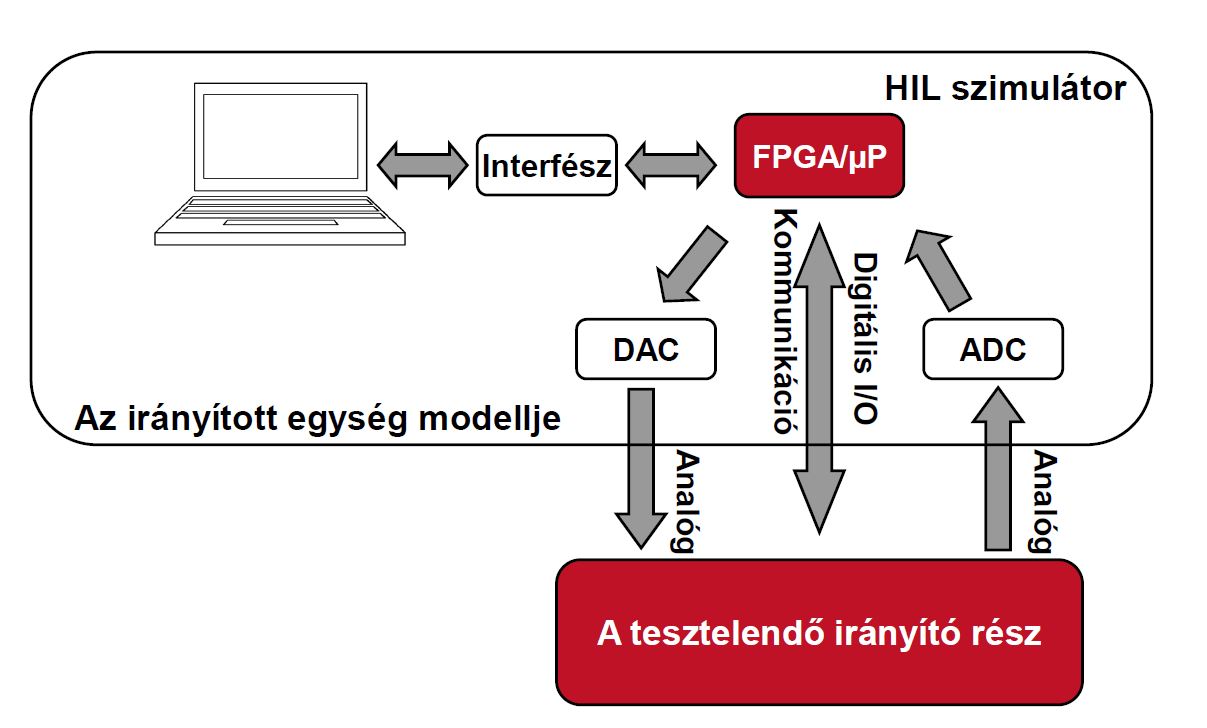
\includegraphics[width = 0.8\textwidth]{figures/hil_idea.png}
	\caption{Az FPGA alapú HIL szimulátor felépítése} 
	\label{fig:hil_idea}
\end{figure}

\todo[inline]{Köki ppt-t behivatkozni}

\section{Szimulációs algoritmusok\cite{koki_varjasi}}

Az áramköri szimulációk numerikus megoldása általában differenciálegyenlet rendszerekre vezethetőek vissza. Az irodalom számos megoldásról említést tesz. A legtöbb eseteben a modellezendő szakasz matematikai modelljét felállítjuk egy ismert gerjesztésre adott válasz alapján, majd az így kapott modellt diszkretizáljuk.

Egy általános folytonos idejű rendszert az alábbi egyenletek reprezentálnak: 

\begin{equation}
\begin{align*}
\underline{x}'(t) &= \underline{\underline{A}}\cdot \underline{x}(t) + \underline{\underline{B}}\cdot{}\underline{x}(t) \\[0.3em]
\underline{y}(t) &= \underline{\underline{C}}\cdot \underline{x}(t) + \underline{\underline{D}}\cdot{}\underline{x}(t)
\end{align*} 
\end{equation}

ahol, $\underline{x}$ az állapotváltozók vektora, az $\underline{u}$ a rendszer bemenete, $\underline{y}$ pedig a rendszer által adott válasz.
A legegyszerűbb numerikus megoldó módszer az Euler módszer, mely az állapot változók módosításán alapul, minden lépésben maguk az állapot változók és a bemenet aktuális értéke alapján. A diszkretizált egyenlet rendszer az előrelépő (forward) Euler módszert alkalmazva az alábbi alakot ölti:

\begin{equation}
\begin{align*}
\underline{x}[n + 1] &= (\underline{\underline{A}} \cdot T + \underline{\underline{I}}) \cdot \underline{x}[n] + \underline{\underline{B}}\cdot{}T\cdot{}\underline{x}[n] \\[0.3em]
\underline{y}[n] &= \underline{\underline{C}}\cdot \underline{x}[n] + \underline{\underline{D}}\cdot{}\underline{x}[n]
\end{align*} 
\end{equation}

ahol $\underline{\underline{I}}$ az egység mátrix, $T$ a lépésköz, $n$ pedig az aktuális lépés indexe.Egy másik változata az Euler módszernek a hátralépő (backward) Euler módszer, vagy más néven implicit Euler módszer. A különbség a két módszer között, hogy az implicit Euler az aktuális értékek helyett a következő lépés értékeit használja:

\begin{equation}
\underline{x}[n + 1] = \ x[n] + \underline{\underline{A}} \cdot T \cdot \underline{x}[n + 1] + \underline{\underline{B}}\cdot{}T\cdot{}\underline{u}[n+1] \\[0.3em]
\end{equation}

Mivel $\underline{x}[n+1]$ az egyenlet mindkét oldalán megjelenik, implicit módszerről beszélünk. Átrendezés után az állapot egyenlet az alábbi alakot öltik:

\begin{equation}
\begin{align*}
\underline{x}[n + 1] &= (\underline{\underline{I}} - \underline{\underline{A}} \cdot T )^{-1} \cdot\underline{x}[n] + (\underline{\underline{I}} - \underline{\underline{A}} \cdot T)^{-1} \underline{\underline{B}}\cdot{}T\cdot{}\underline{x}[n + 1] \\[0.3em]
\underline{y}[n] &= \underline{\underline{C}}\cdot \underline{x}[n] + \underline{\underline{D}}\cdot{}\underline{x}[n]
\end{align*} 
\end{equation}

A formulából jól látszik, hogy az aktuális érték kiszámításához szükség van a változók ,,jövőbeni'' értékére. Erre következtethetünk a változók jelenlegi értékéből, vagy további késleltetést adva a rendszerhez összegyűjthetjük a számításhoz szükséges értékeket.
A két korábbi módszer kombinációja, mely széles körben alkalmazott szimulációs eljárások során a következő. Ez a módszer a trapéz módszer, a változók jelenlegi és következő lépésbeli értékek átlagát használja, így jobb közelítést adva, mintha két korábbi értéket használna:

\begin{equation}
\underline{x}[n + 1] = \ x[n] + \frac{1}{2}\underline{\underline{A}} \cdot T \cdot \underline{x}[n + 1] + \frac{1}{2}\underline{\underline{A}}\cdot{}T\cdot{}\underline{x}[n] + \frac{1}{2}\underline{\underline{B}} \cdot T \cdot \underline{u}[n + 1] + \frac{1}{2}\underline{\underline{B}}\cdot{}T\cdot{}\underline{u}[n] \\[0.3em]
\end{equation}

\paragraph{}
Látható, hogy ez szintén egy implicit módszer, hiszen ez is tartalmazza $\underline{x}[n+1]$-et mindkét oldalon, illetve szintén támaszkodik a gerjesztés jövőbeni értékére is. Kifejezve $\underline{x}[n+1]$-et az alábbi alakot kapjuk:

\begin{equation}
\begin{align*}
\underline{x}[n + 1] &= (\underline{\underline{I}} - \frac{1}{2}\underline{\underline{A}} \cdot T )^{-1} \cdot{} (\underline{\underline{I}} + \frac{1}{2}\underline{\underline{A}} \cdot T )^{-1} \cdot{} \underline{x}[n] + (\underline{\underline{I}} - \frac{1}{2}\underline{\underline{A}} \cdot T)^{-1} \cdot{} \\ (\frac{1}{2}\underline{\underline{B}} \cdot{} T \cdot{} \underline{u}[n+1] + \frac{1}{2}\underline{\underline{B}} \cdot{} T \cdot{} \underline{u}[n])  \\[0.3em]
\underline{y}[n] &= \underline{\underline{C}}\cdot \underline{x}[n] + \underline{\underline{D}}\cdot{}\underline{x}[n]
\end{align*} 
\end{equation}

\paragraph{}
Az összes módszer mátrix műveletekre vezethető vissza, az implementációjukhoz csupán mátrix szorzásra és összeadásra van szükség. Egy olyan szimulátor, amely általános állapot egyenletek megoldására képes, igen rugalmas tud lenni, a mátrixok együtthatóinak változtatásával, különböző rendszerek szimulációit hozhatjuk létre. További numerikus integráláson alapuló algoritmusok is állnak rendelkezésre, de ezek már másodrendű módszerek, amely azt jelenti, hogy szükségük van az állapot változók.
\paragraph{}
Szintén gyakran használt közelítő algoritmus a negyed rendű Runge-Kutta módszer, mely a numerikus integrálástól eltérő megközelítést alkalmaz.

\begin{equation}
\begin{align*}
\underline{a}[n] &= \underline{\underline{A}}\cdot \underline{x}[n] + \underline{\underline{B}}\cdot{}\underline{u}[n] \\[0.3em]
\underline{b}[n] &= \underline{\underline{A}}\cdot (\underline{x}[n] + \frac{1}{2}T \cdot \underline{a}[n]) + \underline{\underline{B}}\cdot{}\underline{x}[n + 0,5] \\[0.3em]
\underline{c}[n] &= \underline{\underline{A}}\cdot (\underline{x}[n] + \frac{1}{2}T \cdot \underline{b}[n]) + \underline{\underline{B}}\cdot{}\underline{x}[n + 0,5] \\[0.3em]
\underline{d}[n] &= \underline{\underline{A}}\cdot (\underline{x}[n] + T \cdot \underline{c}[n]) + \underline{\underline{B}}\cdot{}\underline{x}[n + 1] \\[0.3em]
\underline{x}[n+1] &= \underline{x}[n] + \frac{1}{6}T \cdot{} (\underline{a}[n] + 2 \cdot{} \underline{b}[n] + 2 \cdot{} \underline{c}[n] + \underline{d}[n]) \\[0.3em]
\underline{y}[n] &= \underline{\underline{C}} \cdot{} \underline{x}[n] + \underline{\underline{D}} \cdot \underline[n]
\end{align*} 
\end{equation}

ahol $\underline{a}$, $\underline{b}$, $\underline{c}$, és $\underline{d}$ csak ideiglenesen használt vektorok. Ennek az algoritmusnak nem csak a gerjesztés következő értékére, hanem a két lépés közötti ($\underline{u}[n+0,5]$), melyet könnyedén megoldhatunk a bemenet kétszeres frekvenciájú mintavételezésével, vagy a két egymást követő érték átlagának kiszámításával.